\section{Pada Website}
Ini biasanya terjadi pada saat melakukan pull request. Tertulis pada website ada konflik seperti gambar \ref{fig:webkonflik1}. 

\begin{figure}[!htbp]
\centerline{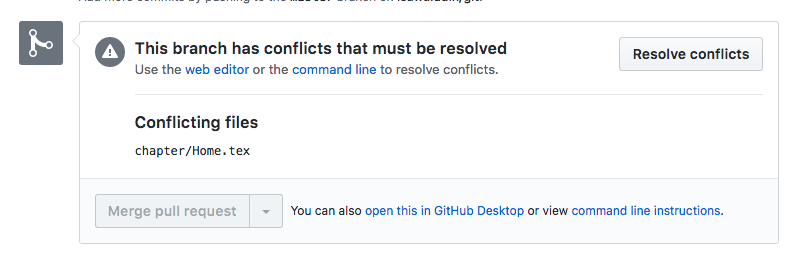
\includegraphics[width=.75\textwidth]{Figures/webkonflik1}}
\caption{Konflik Pada Saat Pull Request}
\label{fig:webkonflik1}
\end{figure}

Tetap tenang, ini sangatlah mudah untuk dilakukan solusinya yaitu dengan merge. Pertama kita klik Resolve conflicts yang terlihat pada gambar \ref{fig:webkonflik1}. Merge adalah proses memilih salah satu atau menggabungkan bagian yang ditandai oleh git. Sebagai contoh misalnya di gambar \ref{fig:webkonflik3}, tertulis ada 4 konflik. 

\begin{figure}[!htbp]
\centerline{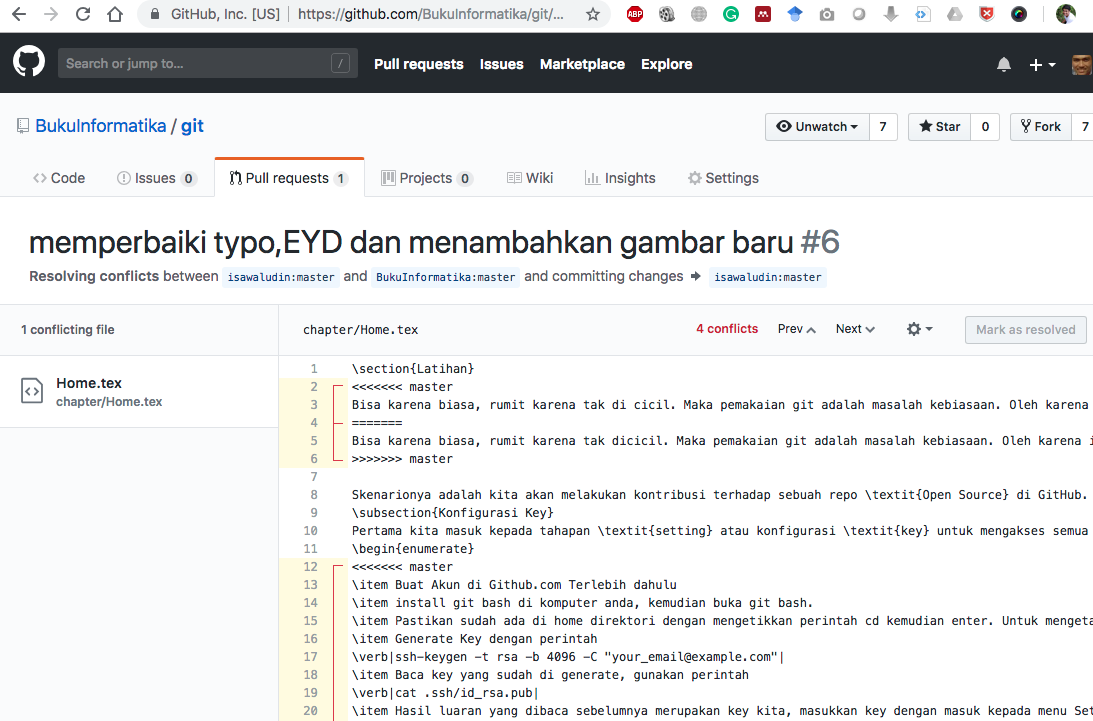
\includegraphics[width=.75\textwidth]{Figures/webkonflik3}}
\caption{Konflik Pada Saat Pull Request}
\label{fig:webkonflik3}
\end{figure}

Konflik yang pertama pada tulisan \textit{Bisa karena biasa....}. Maka kita tinggal melakukan merging dengan cara memilih kata pada baris ketiga atau kelima, atau bisa juga menggabungkan keduanya, jika memang isinya berbeda atau memodifikasi lagi. Setelah memilih jangan lupa menghapus tanda konflik seperti yang terlihat pada baris 2,4 dan 6. Baris 2 artinya itu tanda mulai, baris 6 artinya itu tanda akhir, dan baris 4 itu tanda untuk memilih apakah yang atas atau yang bawah. Sehingga definisi merge pada konflik ini terlihat pada gambar \ref{fig:webkonflik5}.



\begin{figure}[!htbp]
\centerline{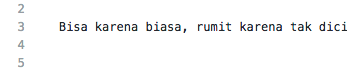
\includegraphics[width=.75\textwidth]{Figures/webkonflik5}}
\caption{Hasil Merge Setelah memilih dan menghapus tanda}
\label{fig:webkonflik5}
\end{figure}



